\documentclass[tikz, border=4pt]{standalone}
\usepackage{tikz}
\usetikzlibrary{calc}
\definecolor{tuerkis}{HTML}{D9EEEE}
\definecolor{antituerkis}{HTML}{FFE5CF}
\definecolor{darkantituerkis}{HTML}{FF9A0C}
\definecolor{RoyalBlue}{RGB}{22,111,191}

\begin{document}
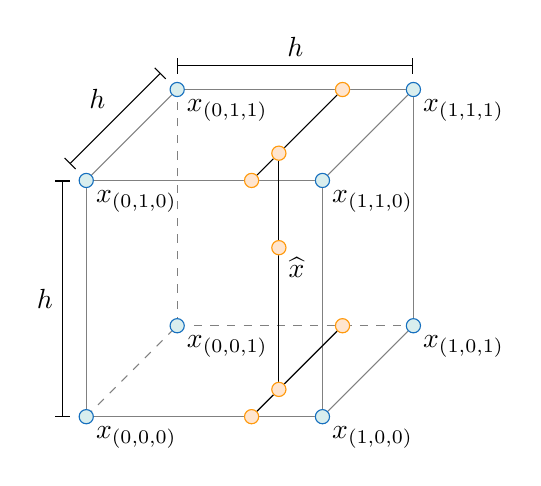
\begin{tikzpicture}[scale=3, z=.385cm]
    \foreach [count=\i from 0] \n in  {(0,0,0),(0,1,0),(0,0,1),(0,1,1),(1,0,0),(1,1,0),(1,0,1),(1,1,1)}
    \draw \n coordinate (n\i);

    \draw [gray] (n3) -- (n7);
    \draw [gray] (n6) -- (n7);
    \draw [gray] (n0) rectangle (n5);
    \draw [dashed, gray] (n0) -- (n2);
    \draw [dashed, gray] (n2) -- (n6);
    \draw [dashed, gray] (n2) -- (n3);
    \draw [gray] (n4) -- (n6);
    \draw [gray] (n1) -- (n3);
    \draw [gray] (n5) -- (n7);

    \coordinate (o0) at (.7,0,0);
    \coordinate (o1) at (.7,0,1);
    \coordinate (o2) at (.7,1,0);
    \coordinate (o3) at (.7,1,1);

    \draw (o0) -- (o1);
    \draw (o2) -- (o3);

   \draw ($(o0)!.3!(o1)$) coordinate (p0) -- ($(o2)!.3!(o3)$) coordinate (p1);

    \foreach \x in {o0,o1,o2,o3,p0,p1} {
      \filldraw [antituerkis] (\x) circle (.03);
      \draw [darkantituerkis] (\x) circle (.03);
    }

    \foreach \n in  {(0,0,0),(0,1,0),(0,0,1),(0,1,1),(1,0,0),(1,1,0),(1,0,1),(1,1,1)}
    \draw \n node [black, below right] {$\bm{x}_{\n}$};
    \foreach \i in {0,1,...,7}
    {
%      \draw let \p{X}=(n\i) in node [black, fill=white, below right] {$\bm{x}$};
      \filldraw [tuerkis] (n\i) circle (.03);
      \draw [RoyalBlue] (n\i) circle (.03);
    }
    \draw [|-|] ($(n0)-(.1,0,0)$) -- node [left] {$h$} ($(n1)-(.1,0,0)$);
    \draw [|-|] ($(n3)-(0,-.1,0)$) -- node [above] {$h$} ($(n7)-(0,-.1,0)$);
    \draw [|-|] ($(n1)-(.07,-.07,0)$) -- node [above left] {$h$} ($(n3)-(.07,-.07,0)$);

    \filldraw [antituerkis] ($(p0)!.6!(p1)$) circle (.03);
    \draw [darkantituerkis] ($(p0)!.6!(p1)$) circle (.03) node [black, below right] {$\widehat{\bm{x}}$};
  \end{tikzpicture}
\end{document}
